\documentclass[12pt,openany,a4paper, titlepage]{article}

%import package
\usepackage[utf8]{inputenc}
\usepackage[T1]{fontenc}
\usepackage{lmodern}
\usepackage[french]{babel}
\usepackage{amsfonts,amsmath,amssymb,amsthm}
\usepackage{geometry} %fix the margin of the document
\geometry{top=3cm, bottom=3cm, left=2.5cm, right=2.5cm}
\usepackage{xargs}    %define new command
\usepackage{graphicx} %insertion image
\usepackage{caption}  %insertion de légendes et titres
\usepackage{indentfirst}
\usepackage{color}
\usepackage[table]{xcolor}
\usepackage{float}
\usepackage{tcolorbox}
\usepackage{appendix} % Appendices


% Bibliographie
\usepackage[backend=biber,sorting=nyt,citestyle=authoryear,bibstyle=alphabetic]{biblatex}% Bibliographie
\addbibresource{biblio.bib} 
\usepackage{csquotes}
\usepackage{url}

%title shape %\MakeUppercase
\usepackage{titlesec}
\titleformat{\chapter}[display]
{\normalfont\huge\bfseries\center}{\chaptertitlename\ \thechapter}{20pt}{\Huge}
\titleformat{\section}
{\normalfont\Large\bfseries\center}{\thesection}{1em}{}
\titleformat{\subsection}
{\normalfont\large\center}{\thesubsection}{1em}{}
\titleformat{\subsubsection}
{\normalfont\normalsize\bfseries\center}{\thesubsubsection}{1em}{}
\titleformat{\paragraph}[runin]
{\normalfont\normalsize\bfseries}{\theparagraph}{1em}{}
\titleformat{\subparagraph}[runin]
{\normalfont\normalsize\bfseries}{\thesubparagraph}{1em}{}

%news commands
\newcommand{\f}[2]{\frac{#1}{#2}}
\newcommand{\lp}{\left(}
\newcommand{\rp}{\right)}
\newcommand{\lb}{\left|}
\newcommand{\rb}{\right|}
\newcommand{\lc}{\left[}
\newcommand{\rcc}{\right]}
\newcommand{\la}{\left\langle}
\newcommand{\ra}{\right\rangle}
\newcommand{\dd}{\;\mathrm{d}}
\newcommand{\ddt}[1]{\frac{\partial #1}{\partial t}}
\newcommand{\R}{\mathbb{R}}
\newcommand{\C}{\mathbb{C}}
\newcommand{\Z}{\mathbb{Z}}
\newcommand{\N}{\mathbb{N}}
\newcommand{\HH}{\mathcal{H}}
\newcommand{\spec}{\operatorname{spec}}
\newcommand{\res}{\operatorname{res}}
\newcommand{\specp}{\operatorname{spec_p}}
\newcommand{\essran}[1]{\operatorname{ess_{#1}ran}}
\newcommand{\esssup}[1]{\operatorname{ess_{#1}sup}}
\newcommand{\rd}{\mathbb{R}^d}
\newcommand{\vp}{\varphi}
\newcommand{\He}{H(\epsilon)}
\newcommand{\inv}{^{-1}}
\newcommand{\St}[2]{e^{-i #1 #2}}
\newcommand{\Stt}[2]{e^{i #1 #2}}
\newcommand{\ortho}{P^\perp}
\newcommand{\Ker}{\operatorname{Ker}}
\newcommand{\im}{\operatorname{Im}}
\newcommand{\pvm}{\mathrm{d}\langle \rangle}
\newcommand{\suminf}[2]{\sum_{#1=#2}^{+\infty}}

%new sections
\newtheorem{Def}{Définition}
\newtheorem{defprop}{Définition/Proposition}
\newtheorem{prop}{Proposition}
\newtheorem{theo}{Théorème}
\newtheorem{lem}{Lemme}
\theoremstyle{definition}
\newtheorem{ass}{Hypothèses}
\newtheorem{cor}{Corollaire}
\theoremstyle{definition}
\newtheorem{Not}{Notation}
\theoremstyle{definition}
\newtheorem{ex}{Exemple}
\theoremstyle{definition}
\newtheorem{exs}{Exemples}
\theoremstyle{definition}
\newtheorem{rem}{Remarque}
\newtheorem{postulat}{Postulat}
\theoremstyle{definition}


\everymath{\displaystyle}

\title{La règle d'or de Fermi}
\author{Théo Duez }

%\begin{figure}
%    \begin{minipage}[c]{.46\linewidth}
%       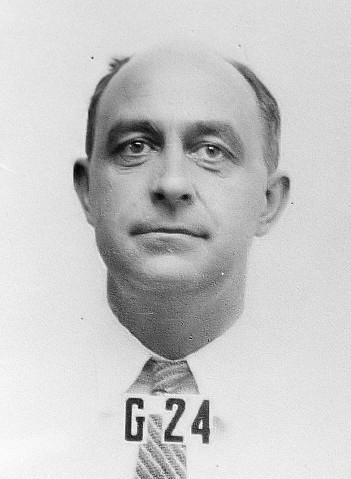
\includegraphics[height=6cm]{Enrico_Fermi.png} 
%        \caption{"Enrico Fermi"}
%    \end{minipage} \hfill
%    \begin{minipage}[c]{.46\linewidth}
%        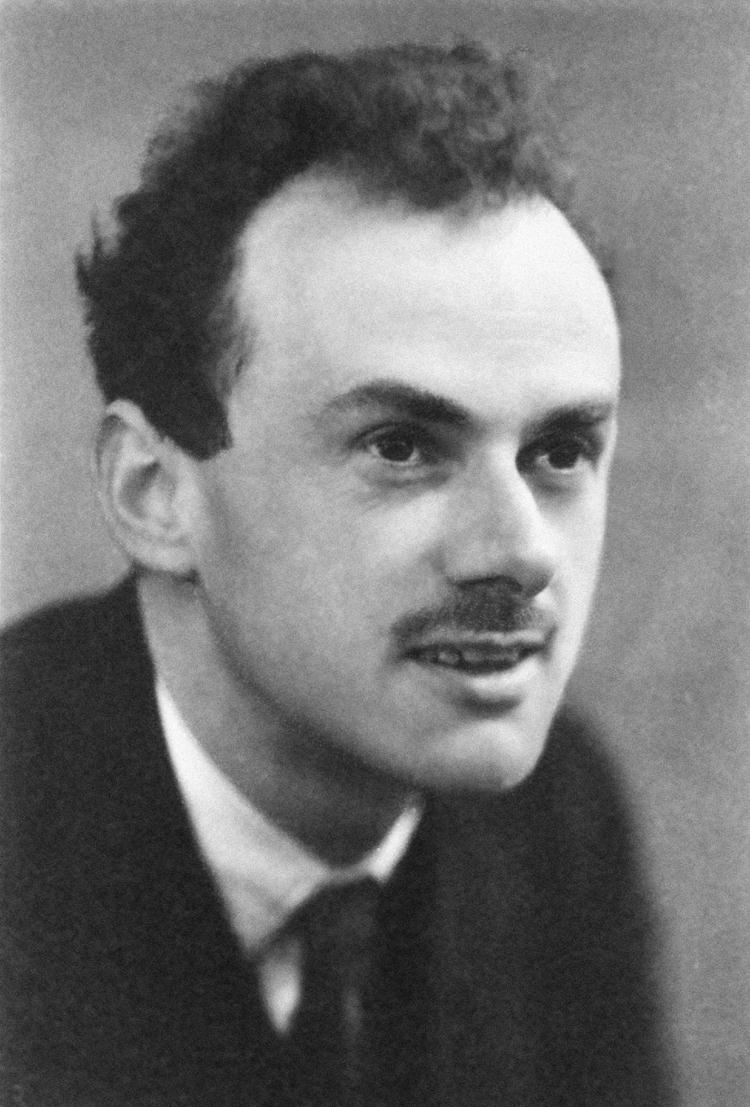
\includegraphics[height=6cm]{Paul_Dirac.jpg}
%        \caption{"Paul Dirac"}
%    \end{minipage}
%\end{figure}


\begin{document}


\maketitle

\newpage

\tableofcontents

\newpage

\section{Introduction}

\subsection{La mécanique quantique}

Développé dans les années par une dizaine de physiciens devenus célèbres dont notamment Paul Dirac, Werner Heisenberg, Louis de Broglie, Erwin Schrödinger etc.,  la mécanique quantique est la branche de la physique théorique qui permet d'expliquer le comportement des particules élémentaires, des atomes, des molécules ou de tout système physique de taille similaire. Elle a rencontré de nombreux succès en permettant d'expliquer ce que la physique classique ne pouvait pas, par exemple la structure électronique des atomes et des molécules, .... . 

Nous ne prétendons pas ici à fournir ne serait-ce qu'une introduction d'introduction d'un vrai cours de mécanique quantique, et bon nombre de concepts et de résultats élémentaires seront omis. Pour plus de détails, nous renvoyons le lecteur à [], [] ou []. Nous allons juste nous concentrer sur ce que l'on appelle les postulats de la mécanique quantique qui permettent de poser les bases de la modélisation mathématique et de ses outils avec lesquels nous allons traiter tout au long de ce rapport.

\vspace{3mm}
\begin{tcolorbox}[colback=gray!5!white,
                  colframe=gray!80!white,
                  title= Postulat 1 : Principe de superposition ]
L'état d'un système quantique est défini à tout instant $t$ par un vecteur unitaire, dénoté $|\psi(t)\rangle$, appartenant à un espace de Hilbert complexe $\HH$ séparable. Deux états qui différent d'un facteur de phase $e^{i\theta}$ pour $\theta\in[0,2\pi)$ représentent le même état.
\end{tcolorbox}
\vspace{3mm}

\begin{exs}
    Donnons quelques exemples d'espaces d'états.
    \begin{enumerate}
        \item[1] $\C$ est l'espace de Hilbert séparable le plus simple que l'on puisse considérer. Comme deux complexes de module 1 différent toujours d'un facteur de phase, cet espace est trivial puisque constituer que d'un seul état.
        \item[2] $\C^2$ est quant à lui l'espace non trivial le plus simple que l'on puisse considérer. Soit $|\psi\rangle = (re^{i\vp}, r'e^{i\vp'}) \in \C^2$ avec $r,r'\geq 0$ et $\vp, \vp' \in [0,2\pi)$. Quitte à multiplier par le facteur de phase $e^{-i\vp}$ (qui ne change pas l'état du système, on peut supposer $\vp = 0$. Comme un vecteur d'état est de norme 1, on a que $r^2 + r'^2 = 1$ et il existe donc $\theta \in [0,2\pi[$, que l'on peut réduire à $\theta \in [0,\pi[$ une nouvelle fois par invariance par multiplication par un facteur de phase, tel que $|\psi\rangle = \lp \cos(\theta), \sin(\theta)e^{i\vp}\rp$. Une telle paramétrisation fait que l'on appelle cet espace d'état la sphère de Bloch, qui permet de modéliser par exemple les qubits, composants de base en thérie de l'information quantique.
        \item[3] De même, on peut considérer $\C^n$ pour $n\in\N$. Un tel espace peut modéliser un système qui peut se déplacer/propager sur un ensemble de $n$ sites.
        \item[4]  De façon plus général, si l'on souhaite considérer un système qui évolue sur une chaîne discrète infinie, l'espace approprié à considérer est $\ell^2(\Z)$, l'espace des suites sur $\Z$ de carré intégrable, qui est bien, muni sa norme euclidienne, un espace de Hilbert séparable. On peut aussi considérer $\ell^2(A)$ où $A$ est un ensemble dénombrable.
        \item[5] Un dernier exemple est l'espace $L^2(\R^d,\C)$ où $d\in\N$, l'espace des fonctions de $R^d$ vers $\C$ de carré intégrable. Cet espace est un espace de Hilbert séparable pour sa norme euclidienne. C'est l'espace typique utiliser si l'on souhaite par exemple modéliser un système dont la position varie dans un continuum, ici $\R^d$.
    \end{enumerate}
\end{exs}

\vspace{3mm}
\begin{tcolorbox}[colback=gray!5!white,
                  colframe=gray!80!white,
                  title= Postulat 2 : Principe de correspondance ]
A tout observable classique correspond un opérateur linéaire $A$ autoadjoint sur $\HH$.
\end{tcolorbox}
\vspace{3mm}

\begin{rem}
    $A$ est simplement une matrice si $\HH$ est de dimension finie mais peut être un opérateur possiblement non borné si $\HH$ est de dimension infinie. L'étude de tels opérateurs, et à l'instar des matrices de leur spectre et diagonalisabilité, fait l'objet de la théorie dite spectrale dont nous ferons un très rapide tour dans la section suivante. Ici autoadjoint est une généralisation à la dimension infinie de la notion d'hermitianité pour les matrices complexes.
\end{rem}

\begin{ex}
    
\end{ex}


\vspace{3mm}
\begin{tcolorbox}[colback=gray!5!white,
                  colframe=gray!80!white,
                  title= Postulat 3 : Principe de quantification ]

\end{tcolorbox}
\vspace{3mm}

\vspace{3mm}
\begin{tcolorbox}[colback=gray!5!white,
                  colframe=gray!80!white,
                  title= Postulat 4 : Principe de décomposition spectrale ]

\end{tcolorbox}
\vspace{3mm}

\vspace{3mm}
\begin{tcolorbox}[colback=gray!5!white,
                  colframe=gray!80!white,
                  title= Postulat 5 : Principe de réduction du paquet d’onde ]

\end{tcolorbox}
\vspace{3mm}

\vspace{3mm}
\begin{tcolorbox}[colback=gray!5!white,
                  colframe=gray!80!white,
                  title= Postulat 6 : Evolution d'un système dans le temps ]
Entre toute mesure, l'évolution de l'état d'un système quantique est régit par l'équation de Schrödinger 
$\partial_t \psi(t) = H(t)\psi(t)$
où $H(t)$ est l'opérateur correspondant à l'hamiltonien du système à l'instant $t$, i.e à l'observable "énergie total".
\end{tcolorbox}
\vspace{3mm}

\begin{rem}
    \begin{enumerate}
        \item[1] L'opérateur $H$, correspondant à une observable classique, est un opérateur auto-adjoint.
        \item[2] L'existence de solutions à un tel équation est donné par le théorème de Stone que nous verrons dans la section suivante sur les rappels de théorie spectrale.
    \end{enumerate}
\end{rem}

\begin{exs}
    
\end{exs}

\subsection{La règle d'or de Fermi} 

Qu'est ce que la règle d'or de Fermi ? A ce propos, Wikipédia [] dit efficacement ceci : \\

\begin{it}
    "En physique quantique, la règle d'or de Fermi est un moyen de calculer le taux de transition (probabilité de transition par unité de temps) à partir d'un état propre énergétique d'un système quantique vers un continuum d'états propres, par perturbation."
\end{it}\\

Cette définition mérite un certains nombres d'explications que nous allons  prendre le temps de donner. 

\paragraph{Spectre continue}
Comme nous l'avons rappelé, tout système quantique est régit par un opérateur linéaire, appelé Hamiltonien et noté $H$, auto-adjoint. Cet opérateur peut agir soit sur des espaces  de dimension fini, dans ce cas $H$ est simplement une matrice, ou des espaces de dimension infinies, à tire d'exemple citons le Laplacien agissant sur $H^2(\R^3)$. Les grandeurs qui peuvent être mesurées sur ce systèmes sont les valeurs propres de cet opérateur, le système se projetant alors sur le sous-espace propre associé. S'il est aisé d'étudier le spectre de matrice, étudier le spectre d'opérateur de dimension infini est plus délicat et se traire dans des cours de Théorie Spectrale. Nous renvoyons en annexe à quelques définitions et grands principes de la théorie spectrale et supposerons que le lecteur a connaissance des notions abordés dans l'annexe. Il est important de noter que la théorie spectrale en dimension infinie est certes plus général que celle de la dimension finie, mais implique nombre de résultats et de notions plus délicates qui sont complètement absents du monde fini-dimensionnel et qui ne peuvent donc pas être "intuité". Illustrons cela.
- spectre opérateur compact, opérateurs continues -> cela vient du fait que différence injective <=> bijective <=> surhective
L'hamiltonien $H$ possède la propriété d'être auto-adjoint. Il s'agit là d'une généralisation d'être symétrique pour des matrices réelles ou hermitiennes pour des matrices complexes. Il est possible de montrer qu'il est possible de daignoliser, dans un sens généraliser, tout opérateurs auto-adjoints, dont les valeurs propres sont alors réelles. Nous renvoyons encore ici à l'annexe pour plus de détails. Cette hypothèse qui vient des physiciens est assea naturel si l'on cherche à faire les postulats [] et [].

\paragraph{Pertubation}
Expliquons maintenant ce que l'on entend par perturbation en phsyique quantitique. Il arrive souvent que le système que l'on étudie est soumise à une "petite" perturbation, c'est à dire que notre hamiltonien de départ se retrouve remplacé par un nouvel hamitonien $H(\epsilon) := H_0 + \epsilon H_1$ où $H_1$ est aussi un opérateur autoadjoint représentant la perturbation et $\epsilon$ un réel positif qui a vocation a être petit.  Par exemple, cela peut modéliser []. En présence de tels perturbations, les valeurs propres initiales peuvent se retouver pertuber, et la connaissance des valeurs propres étant fondamentales en phsyiqye quantique, des physiciens ont développé des théories pour calculer, étudier, caractérisé les valeurs propres perturbées et qui ont été reprises rigoureusement par des mathématiciens comme la théorie de Kato qui stipule de nombreux résultats selon la régularité des domaines des opérateurs $H_0$ et $H_1$. 

\paragraph{Pertubation}


En résumé, 

\subsection{Objectifs de ce projet}

Comme nous l'avons dit, la règle d'or de Fermi est un résulta bien connue des physiciens. Toutefois, les preuves que l'on peut trouver dans des livres de physiques reposent souvent sur des hypothèses pas toujours claires voire douteuse. A tire d'exemple, Wikipédia [] propose une preuve dans le paragraphe qui fait une hypothèse qui n'est pas clair. Les mathémaciens, comme souvent, ont cherché à justifier rigoureussement les assertions des physiciens et sont parvenu à établir des résultats sur la règle d'or de Fermi. L'objectif de ce projet est donc d'étudier différentes preuves permettant d'établir la règle d'or de Fermi. Nous investigureons deux approches très différents, une dite par les résonnances, qui reposent sur de nombreux concepts de théorie spectrale, et sur l'approche de Davies qui repose sur l'étude d'un problème d'évolution. Nous chercherons à expliciter et simplifier ces démonstrations  dans le cas de systèmes quantiques simples ainsi qu'à comparer ces deux approches. Nous proposons aussi l'étude de [dimension finie]. 

\section{Introduction of the main Mathematical tools}

Pour étudier la règle d'or de Fermi, et les problèmes de mécaniques quantiques en général, les mathématiciens ont recours à une théorie fondamentale : la théorie spectrale. Cette théorie a pour but d'étudier le comportement d'opérateurs linéaires sur des espaces de Hilbert ou de Banach potentiellement (et surtout ) de dimension infinie, et de leurs spectres, généralisant les études bien connues sur les matrices, opérateur de dimension finie. 

[Continuer intro]

Il faut un cours entier de M2 pour établir les éléments introductifs de la théorie spectrale et commencer à entrevoir les théorie sous-jacente, comme la théorie des perturbations de Kato, le principe du maximum ou la théorie de la diffusion. Cette théorie requiert 

\subsection{Premières définitions} (1 Pages)

- Déf opérateur, bornée, non-bornée, symétrique
- Déf adjoint d'un opérateur, déf autoadjoint (généralisation de Hermitienne)
- Exemples

\subsection{Spectre et Résolvant} (1.5 pages)

- Déf résolvant, spectre et différents types de spectre
- Identité du résolvant
- Opérateur conjugué => même spectre
- Spectre opérateur compact, auto-adjoint (juste propriétés), quelques inégalité et petit principe du maximum


\subsection{Calculs fonctionnels} (1.5 pages)

Intro pour dire pourquoi on s'intéresse à ca : e(iH), généralisation du spectre d'un opérateur T
- Déf convergence forte généralisée

\subsection{Schrodinger-equations}



\newpage
\section{Approche par les résonances}

Dans cette partie, nous abordons l'approche dite par les résonances, dénomination que nous expliquerons dans la suite. Nous reprenons les notations fixées précédemment ([]). L'idée est d'utiliser les formules de Cauchy de théorie spectrale pour se ramener à un problème avec une intégrale complexe. Si $H_0$ est un opérateur bornée de $\mathcal{H}$ dans $\mathcal{H}$ alors son spectre est borné, plus précisément $\spec H_0 \subseteq \lc-||H_0||, ||H_0||\rcc$. La théorie des perturbations classique indique que le spectre de $H(\epsilon$ est "proche" du spectre de $H_0$ lorsque $\epsilon$ est petit. Il existe donc un contour $\Gamma$ dans $\C$ tel que $\spec H \subset int(\Gamma)$ où $int(\Gamma)$ est l'unique composante connexe bornée  de $\C\setminus \Gamma$. On écrit donc d'abord (voir []) :

\begin{equation}
    \la \vp_0 | e^{-i\He t} \vp_0\ra = \f{1}{2i\pi}\oint_\Gamma e^{-itz}\la \varphi_0,\lp H(\epsilon)  -z \rp^{-1} \varphi_0 \ra dz.
\end{equation}

On a remplacé l'étude sur l'exponentielle de $\He$ en une étude de sa résolvante.
\newpage
\subsection{Matrice de Livsic}

Nous abordons dans cette partie la notion de matrice de Livsic qui a été introduite en 1957 par M.S Livsic [], et qui a été redécouvert de nombreuses fois sous différents noms par les physiciens. Il s'agit de la version infini-dimensionnelle de la notion complément de Schur dont nous ferons un parallèle dans la suite. Considérons un opérateur $H$ auto-adjoint sur un espace de Hilbert $\HH$, $E_0$ un sous-espace vectoriel de dimension finie de $\HH$, et $P$ la projection orthogonal sur ce sous-espace. La matrice de Livsic est un outil central pour l'approche par les résonances et de façon informel s'agit d'une matrice $B(z)$ dépendant de la variable complexe $z$ qui permet de réécrire la compression $P(H-z)\inv P = (B(z) -z)\inv$. Ainsi, en donnant une formule explicite à cette matrice, nous pourrons étudier de façon explicite le fait que l'on s'intéresse au bloc $(E_0,E_0)$ dans la décomposition $E_0\oplus E_0^\perp$ de la résolvante de $H$.

Faisons un petit rappel sur la résolvante notée $R(z) := (H-z)\inv$. Cette quantité est bien définie sur le complémentaire du spectre de $H$ et y ait holomorphe. A l'instar des différents types de singularités en analyse complexe, cette quantité est méromorphe sur une certaine partie du spectre : le spectre discret. Pour rappel, le spectre discret $\spec_d H$ est l'ensemble des valeurs propres de multiplicité finie de $H$. La résolvante est donc méromorphe sur le spectre essentiel $\spec_{ess} H = \spec H\setminus\spec_d H$. La compression $PR(z)P$ est donc aussi méromorhpe sur  $\spec_{ess} H$.

Commençons par établir l'existence d'une telle matrice $B(z)$. Celle-ci repose sur le faire que la compression $PR(z)P$ est un opérateur de dimension finie, i.e une matrice, et la proposition suivante.

\begin{prop}
    $PR(z)P$ est inversible pour $z\in\C\setminus\R$.
\end{prop}
\begin{proof}
    D'après la remarque précédente, il suffit donc de montrer que cette quantité est injective. Soit $z = a+ib\in\C\setminus\R$ et $x\in E_0$ tel que $PR(z)Px = 0$. En particulier, on a 

    $$0 = \im\la x\,,\, PR(z)Px \ra = \im\la x\,,\, R(z)x \ra = b\lb\lb\lp (H-a)^2 + b^2 \rp^{-1/2}x\rb\rb^2$$
    car $x = Px$, et car $P$ et $H$ sont auto-adjoint. Comme $b$ est non nul, nécessairement $x = 0$.
\end{proof}

Cela nous permet de définir la notion de matrice de Livsic.

\begin{Def}[Matrice de Livsic]
Pour $z\in \C\setminus\R$, on définit la matrice de Livsic par
\begin{equation*}
    B(z) := (PR(z)P)\inv + z
\end{equation*}
qui vérifie l'identité 
\begin{equation*}
    (B(z)-z)\inv = P(H-z)\inv P.
\end{equation*}
Cet identité nous permet d'étendre la définition de $B(z)$ sur $\C\setminus\spec_{ess} H$.
\end{Def}

Nous avons les deux propriétés suivantes.

\begin{rem}
Cette notion de matrice de Livsic fait écho avec sa version finie dimensionnelle bien connue : le complément de Schur.  
Soient $n,m \in\N^*$. Considérons une matrice $A\in\C^{(n+m)\times (n+m)}$ hermitienne s'écrivant 
\begin{equation*}
    A:= \begin{pmatrix}
A_{11} & A_{12} \\
A_{21} & A_{22} 
\end{pmatrix}
\end{equation*}
avec $A_{11}\in\R^{n\times n},  A_{12}\in\C^{n\times m}, A_{21}\in\C^{m\times n}$ et $A_{22}\in\C^{m\times m}$. Soit $\lambda \in \R$ et cherchons à résoudre le problème aux valeurs propres $Ax = \lambda x$ d'inconnue $x\in\R^{n+m}$ en supposant que $\lambda$ ne soit pas valeur propre de $A_{22}$. La deuxième ligne de ce système conduit à l'égalité $x_2 = -(A_{22}-\lambda)^{-1}A_{21}x_1$ que l'on peut injecter dans la première ligne et obtenir $(A_{11} - A_{12}(A_{22}-\lambda)^{-1}A_{21})x_1 = \lambda x_1 $. On voit que l'on a bien réduit la dimension du problème de départ et que $\lambda$ est valeur propre de $A$ si et seulement si $\lambda$ est valeur propre de $(A_{11} - A_{12}(A_{22}-\lambda)^{-1}A_{21})$.
\end{rem}

\subsection{Théorème de Howland}

Dans son article intitulé \textit{The Livsic  Matrix in Perturbation Theory}, James S. Howland propose en 1975 un théorème de concentration spectrale intéressant, sous l'hypothèse relativement forte mais qui est souvent vérifiée : la possibilité d'effectuer un prolongement analytique de la matrice de Livisc du plan complexe supérieur vers le plan complexe inférieur.

\begin{theo}[\textbf{Concentration spectrale - Howland (1975)}]
Soit $(H_n)$ une suite d'opérateur auto-adjoints convergent fortement dans le sens généralisé vers un opérateur autoadjoint $H$. Soit $\lambda_0$ une valeur propre de $H$ de multiplicité finie et soit $E_0 = \Ker(H -\lambda_0)$. Soient $B_n(z)$  et $B(z) = \lambda_0 I_m$ les matrices de Livsic sur $E_0$ pour $H_n$ et $H$ respectivement. 
Supposons que \begin{enumerate}
    \item[(1)] pour tout $n\in\N$, $B_n(z)$ possède un prolongement analytique $B_n^+(z)$ du plan complexe supérieur sur un voisinage $ \Omega$ de $\lambda_0$,
    \item[(2)] $\lp B_n^+(z)\rp$ converge fortement vers $B(z)$ uniformément sur $\Omega$.
\end{enumerate}
Alors, pour $n$ assez grand, l'équation sur $z$ : $\det(B_n^+(z) -z) = 0 $ possède exactement $m$ solutions comptées avec multiplicités dans $\Omega$. De plus, si on note $\xi_k(n) = \lambda_k(n) - i \Gamma_k(n)$ pour $k\in\{1,\cdots,m\}$ ces solutions, et si on choisis une suite $(\delta_k(n))$ de réels positifs de sorte que $\Gamma_k(n) = o(\delta_k(n))$, alors en définissant les intervalles 
$$ J_k(n) = \bigcup_{k=1}^m (\lambda_k(n) - \delta_k(n),\lambda_k(n) + \delta_k(n))$$ alors $P = st-\lim E_n(J_n)$.
\end{theo}

\begin{proof}
Commençons par prouver l'existence des zéros. Par hypothèse, on a que la suite de matrices $(B_n(z))$ converge uniformément sur $\Omega$ vers $B(z)$, ce qui implique, en combinant au fait que le déterminant est continue, que pour $n$ assez grand et tout $z\in\Omega$, $$ |\det (B_n^+(z) - z) - \det (B(z) - z)| < \epsilon = |\det (B(z) - z)| $$ car $|B_n^+(z) - z - (B(z) - z)| \leq ||B_n - B|| \rightarrow 0$. Ceci étant vrai pour tout $z\in\Omega$, ceci est vrai pour tout $z\in\gamma$ où $\gamma$ est un chemin inclu dans $\Omega$ et entourant $\lambda_0$. Comme $\lambda_0$ est l'unique zéro et de multiplicité $m$ de $\det (B(z) - z)$, par théorème de Rouché [], l'équation $\det(B_n^+(z) -z) = 0$ a exactement $m$ solutions comptées avec multiplicité.

\end{proof}

\newpage

\begin{proof}
En utilisant successivement la formule de Cauchy, l'égalité définissant les matrices de Livsic, 
\begin{eqnarray*}
\la \varphi_0,e^{-iH(\epsilon)t}\varphi_0 \ra - \la\varphi_0,e^{-iH_n(\epsilon)t}\varphi_0 \ra &=& \f{1}{2i\pi}\oint_\Gamma e^{-itz}\la \varphi_0,\lp H(\epsilon) -z)^{-1} - (H_n(\epsilon)-z)^{-1} \rp \varphi_0 \ra dz\\
&=& \f{1}{2i\pi}\oint_\Gamma e^{-itz} \lp B(z,\epsilon) -z)^{-1} - (B_n(z,\epsilon)-z)^{-1} \rp dz
\end{eqnarray*}
\end{proof}


\subsection{Orth's Theorem}

\section{Second Approach : Davies's Theory}





\newpage

\appendix
\appendixpage
\addappheadtotoc

\section{Biblio}

- Antoine Levitt : Schur Complement
- Stephane Nonnenmacher : COurs de théorie Spectrale
- Wikipédia %https://fr.wikipedia.org/wiki/R%C3%A8gle_d%27or_de_Fermi

\end{document}